\documentclass[12pt,a4paper]{article}
\usepackage[UTF8]{ctex}
\usepackage{amsmath,amscd,amsbsy,amssymb,latexsym,url,bm,amsthm}
\usepackage{epsfig,graphicx,subfigure}
\usepackage{enumitem,balance}
\usepackage{wrapfig}
\usepackage{mathrsfs,euscript}
\usepackage[usenames]{xcolor}
\usepackage{hyperref}
\usepackage[vlined,ruled,linesnumbered]{algorithm2e}
\usepackage{float}
\usepackage{booktabs}
\usepackage{listings}
\usepackage{color}
\usepackage{caption}

\definecolor{mygreen}{rgb}{0,0.6,0}
\definecolor{mygray}{rgb}{0.5,0.5,0.5}
\definecolor{mymauve}{rgb}{0.58,0,0.82}
\lstset{
 backgroundcolor=\color{white}, 
 basicstyle = \footnotesize,       
 breakatwhitespace = false,        
 breaklines = true,                 
 captionpos = b,                    
 commentstyle = \color{mygreen}\bfseries,
 extendedchars = false,             
 frame =shadowbox, 
 framerule=0.5pt,
 keepspaces=true,
 keywordstyle=\color{blue}\bfseries, % keyword style
 language = Verilog,                     % the language of code
 otherkeywords={string}, 
 numbers=left, 
 numbersep=5pt,
 numberstyle=\tiny\color{mygray},
 rulecolor=\color{black},         
 showspaces=false,  
 showstringspaces=false, 
 showtabs=false,    
 stepnumber=1,         
 stringstyle=\color{mymauve},        % string literal style
 tabsize=4,          
 title=\lstname                      
}

\usepackage{fontspec}
\hypersetup{colorlinks=true,linkcolor=black}

\newtheorem{theorem}{Theorem}
\newtheorem{lemma}[theorem]{Lemma}
\newtheorem{proposition}[theorem]{Proposition}
\newtheorem{corollary}[theorem]{Corollary}
\newtheorem{exercise}{Exercise}
\newtheorem*{solution}{Solution}
\newtheorem{definition}{Definition}
\theoremstyle{definition}

\renewcommand{\thefootnote}{\fnsymbol{footnote}}

\newcommand{\postscript}[2]
 {\setlength{\epsfxsize}{#2\hsize}
  \centerline{\epsfbox{#1}}}

\renewcommand{\baselinestretch}{1.0}

\setlength{\oddsidemargin}{-0.365in}
\setlength{\evensidemargin}{-0.365in}
\setlength{\topmargin}{-0.3in}
\setlength{\headheight}{0in}
\setlength{\headsep}{0in}
\setlength{\textheight}{10.1in}
\setlength{\textwidth}{7in}
\makeatletter \renewenvironment{proof}[1][Proof] {\par\pushQED{\qed}\normalfont\topsep6\p@\@plus6\p@\relax\trivlist\item[\hskip\labelsep\bfseries#1\@addpunct{.}]\ignorespaces}{\popQED\endtrivlist\@endpefalse} \makeatother
\makeatletter
\renewenvironment{solution}[1][Solution] {\par\pushQED{\qed}\normalfont\topsep6\p@\@plus6\p@\relax\trivlist\item[\hskip\labelsep\bfseries#1\@addpunct{.}]\ignorespaces}{\popQED\endtrivlist\@endpefalse} \makeatother

% caption
\counterwithin*{figure}{section}
\counterwithin*{figure}{subsection}
\counterwithin*{figure}{subsubsection}
\renewcommand{\thefigure}{%
  \ifnum\value{subsection}=0
    \thesection.\arabic{figure}%
  \else
    \ifnum\value{subsubsection}=0
      \thesubsection.\arabic{figure}%
    \else
      \thesubsubsection.\arabic{figure}%
    \fi
  \fi
}

\counterwithin*{table}{section}
\counterwithin*{table}{subsection}
\counterwithin*{table}{subsubsection}
\renewcommand{\thetable}{%
  \ifnum\value{subsection}=0
    \thesection.\arabic{table}%
  \else
    \ifnum\value{subsubsection}=0
      \thesubsection.\arabic{table}%
    \else
      \thesubsubsection.\arabic{table}%
    \fi
  \fi
}

\begin{document}
\noindent
\captionsetup[figure]{labelfont={bf},name={Fig.}}
\captionsetup[table]{labelfont={bf},name={Tab.}}
%========================================================================

\noindent\framebox[\linewidth]{\shortstack[c]{
\Large{\textbf{DCP3362 Computer Organization Lab 2}}\vspace{1mm}\\
\footnotesize{\color{blue}$*$ Name: 石育瑋  \quad ID: A073708 \quad Email: stoneonetwo1203@gmail.com}}}

%\begin{center}
%\Large{\textbf{Computer Organization Lab 1}}\vspace{1mm}\\
%\footnotesize{\color{blue}$*$ Name: 石育瑋  \quad ID: A073708 \quad Email: yuwei.shih.tw@gmail.com}
%\end{center}

\section{Architecture diagrams}

\begin{figure}[H]
\centering
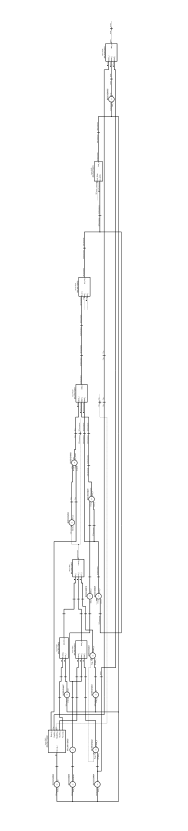
\includegraphics[height=19cm]{fig/dataflow.png}
\caption{Data flow of CPU}
\label{fig:cpu}
\end{figure}

\begin{figure}[H]
\centering
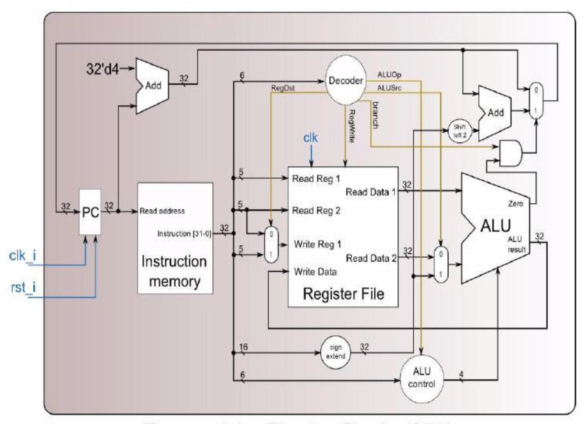
\includegraphics[height=10cm]{fig/cpu.png}
\caption{Architecture}
\label{fig:archi}
\end{figure}


\section{Hardware module analysis}

\begin{enumerate}
\item
在ProgramCounter的設計中:

2個CPU 控制信號:
\begin{itemize}
\item (input) clk$\_$i
\item (input) rst$\_$i
\end{itemize}
rst$\_$i為重置信號;clk$\_$i為clock cycle的控制信號,當clk$\_$i上沿時,(output) pc$\_$out$\_$o進行更新。

\begin{figure}[H]
\centering
\begin{lstlisting}[caption={}]
module ProgramCounter(
    clk_i,
	rst_i,
	pc_in_i,
	pc_out_o
	);
\end{lstlisting}
\caption{ProgramCounter}
\label{fig:alu_top_}
\end{figure}

\item
在Instr$\_$Memory的設計中:
pc$\_$addr$\_$i為輸入指令地址,透過$\$$readmemb讀入我們設定的指令檔案,(output) instr$\_$o 輸出指令。

\begin{figure}[H]
\centering
\begin{lstlisting}[caption={}]
module Instr_Memory(
    pc_addr_i,
	instr_o
	);
\end{lstlisting}
\caption{Instr$\_$Memory}
\label{fig:alu_top_}
\end{figure}

\item
在Decoder的設計中:
\begin{itemize}
\item (input) instr$\_$op$\_$i: 為instruction[31:26]
\item (output) RedWrite$\_$o: 控制是否寫入寄存器
\item (output) ALU$\_$op$\_$o: 提供ALU control
\item (output) ALUSrc$\_$o: 控制ALU source的$2-1$ MUX
\item (output) RegDst$\_$o: 控制選取RD的$2-1$ MUX
\item (output) Branch$\_$o: 控制分支信號
\end{itemize}

\begin{figure}[H]
\centering
\begin{lstlisting}[caption={}]
module Decoder(
    instr_op_i,
	RegWrite_o,
	ALU_op_o,
	ALUSrc_o,
	RegDst_o,
	Branch_o
	);
\end{lstlisting}
\caption{Decoder}
\label{fig:alu_top_}
\end{figure}

%
\item
在Sign$\_$Extend的設計中:
\begin{itemize}
\item (input) data$\_$i: 為16-bit的signed number
\item (output) data$\_$o: 輸出經signed extension之data$\_$i的值
\end{itemize}

\begin{figure}[H]
\centering
\begin{lstlisting}[caption={}]
module Sign_Extend(
    data_i,
    data_o
    );
\end{lstlisting}
\caption{Sign$\_$Extend}
\label{fig:alu_top_}
\end{figure}

%
\item
在Shift$\_$Left$\_$Two$\_$32的設計中:
\begin{itemize}
\item (input) data$\_$i: 為32-bit的number
\item (output) data$\_$o: 輸出左移2-bit 之data$\_$i的值
\end{itemize}

\begin{figure}[H]
\centering
\begin{lstlisting}[caption={}]
module Shift_Left_Two_32(
    data_i,
    data_o
    );
\end{lstlisting}
\caption{Shift$\_$Left$\_$Two$\_$32}
\label{fig:alu_top_}
\end{figure}

%
\item
在Reg$\_$File的設計中:
\begin{itemize}
\item (input) RSaddr$\_$i: RS地址
\item (input) RTaddr$\_$i: RT地址
\item (input) RDaddr$\_$i: RD地址
\item (input) RDdata$\_$i: 要輸入RD的資料
\item (input) RegWrite$\_$i: 是否寫入RD控制信號

\item (output) RSdata$\_$o: RS資料
\item (output) RTdata$\_$o: RT資料
\end{itemize}

\begin{figure}[H]
\centering
\begin{lstlisting}[caption={}]
module Reg_File(
    clk_i,
	rst_i,
    RSaddr_i,
    RTaddr_i,
    RDaddr_i,
    RDdata_i,
    RegWrite_i,
    RSdata_o,
    RTdata_o
    );
\end{lstlisting}
\caption{Reg$\_$File}
\label{fig:alu_top_}
\end{figure}

%%%
\end{enumerate}
\section{Finished part}

除了以上modules的設計之外,還包括連接所有module之間的連線,以及3-bit ALUop自定義。下面是testbench測試出來的波形圖。

\begin{figure}[H]
\centering
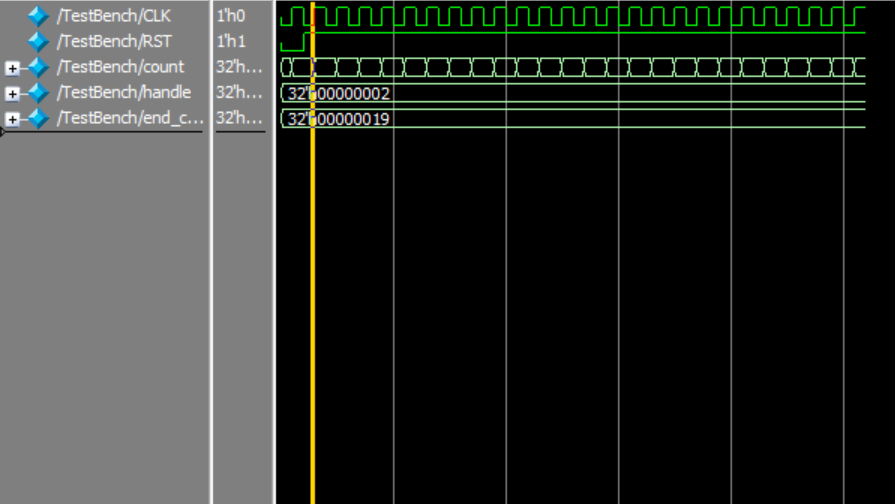
\includegraphics[height=10cm]{fig/res1.png}
\caption{wave1}
\label{fig:archi}
\end{figure}

\begin{figure}[H]
\centering
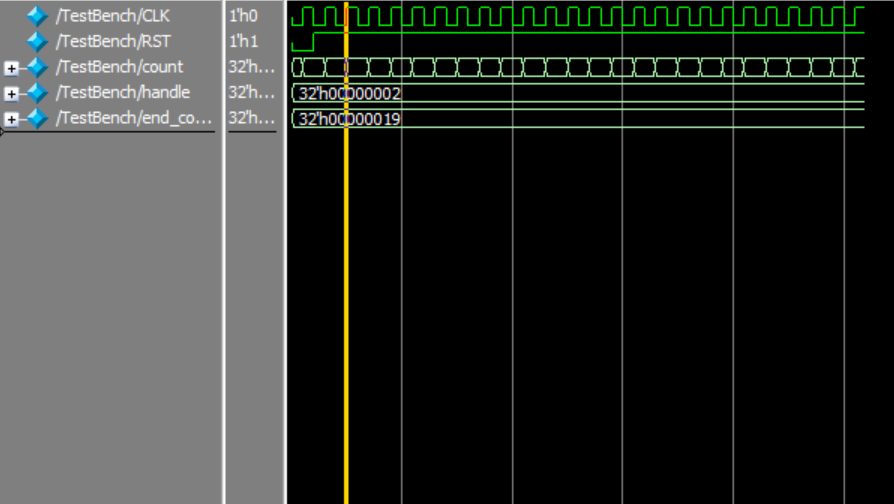
\includegraphics[height=10cm]{fig/res2.png}
\caption{wave2}
\label{fig:archi}
\end{figure}

\section{Problems you met and solutions}

\begin{enumerate}
\item 在組裝所有modules時wire常常連錯,最後參考老師ppt上的架構圖進行連接。
\item 教材裡找不到3-bit的ALUop定義,後面自定義addi等指令。
\end{enumerate}

\section{Summary}

這個Lab很考驗看波形圖debug的能力,才能找出哪裡的線接錯,以及modlue是否有誤。


%========================================================================
\end{document}
